\section{Method}
\label{sec:method}
Here we describe VeriForm, our pipeline for verifying reasoning steps from LLM-generated mathematical step-by-step solutions.

Let $S=(s_1,\ldots,s_n)$ denote a reasoning trace generated by an LLM. We verify each step $s_i$ by routing it to an appropriate verifier $\mathcal{V}$:

$$
\mathcal{R}(s_i)\rightarrow \mathcal{V},
\qquad
\mathcal{V}(s_i)\in\{0,1\},
$$

where $\mathcal{V}(s_i)=1$ indicates that $s_i$ is mathematically correct. The verifier space consists of a Lean verifier $\mathcal{V}*{\mathrm{L}}$, a Python verifier $\mathcal{V}*{\mathrm{P}}$, and a null verifier $\mathcal{V}_{\varnothing}$.

We consider two routing strategies. First, a zero-shot LLM directly predicts the appropriate verifier:

$$
\mathcal{R}_{\mathrm{LLM}}(s_i)
=
\operatorname{LLM}_{\mathrm{route}}(s_i).
$$

Second, we use a BERT-based classifier $\mathcal{C}$ trained to predict the appropriate verifier by minimizing Binary Cross-Entropy (BCE):

$$
\mathcal{R}_{\mathrm{BERT}}(s_i)=\mathcal{C}(s_i).
$$

The Lean verifier is designed for logical reasoning and complex computations. It first maps a natural-language step to a formal statement using an autoformaliser $\mathcal{A}$, and subsequently attempts to prove it using a proof procedure found by a specialised prover $\mathcal{P}$:

$$
s_i\xrightarrow{\mathcal{A}}f_i\xrightarrow{\mathcal{P}}\text{proof}.
$$

The step is accepted if a valid proof is found. The Python verifier targets arithmetic and executable computations. A specialist LLM translates $s_i$ into executable Python code $c_i$, which is then evaluated:

$$
s_i\xrightarrow{\mathcal{G}_{\mathrm{Py}}}c_i\xrightarrow{\mathrm{Exec}}\text{result}.
$$

Finally, $\mathcal{V}_{\varnothing}$ is selected when a step is deemed unsuitable for either verification mechanism, leaving it explicitly unverified.

Thus, the overall procedure applies a specialized verifier to each reasoning step according to the routing decision:

$$
s_i\rightarrow\mathcal{R}(s_i)\rightarrow\mathcal{V}(s_i),
\qquad i=1,\ldots,n.
$$

Figure \ref{fig:placeholder} summarise our method.

\begin{figure}
    \centering
    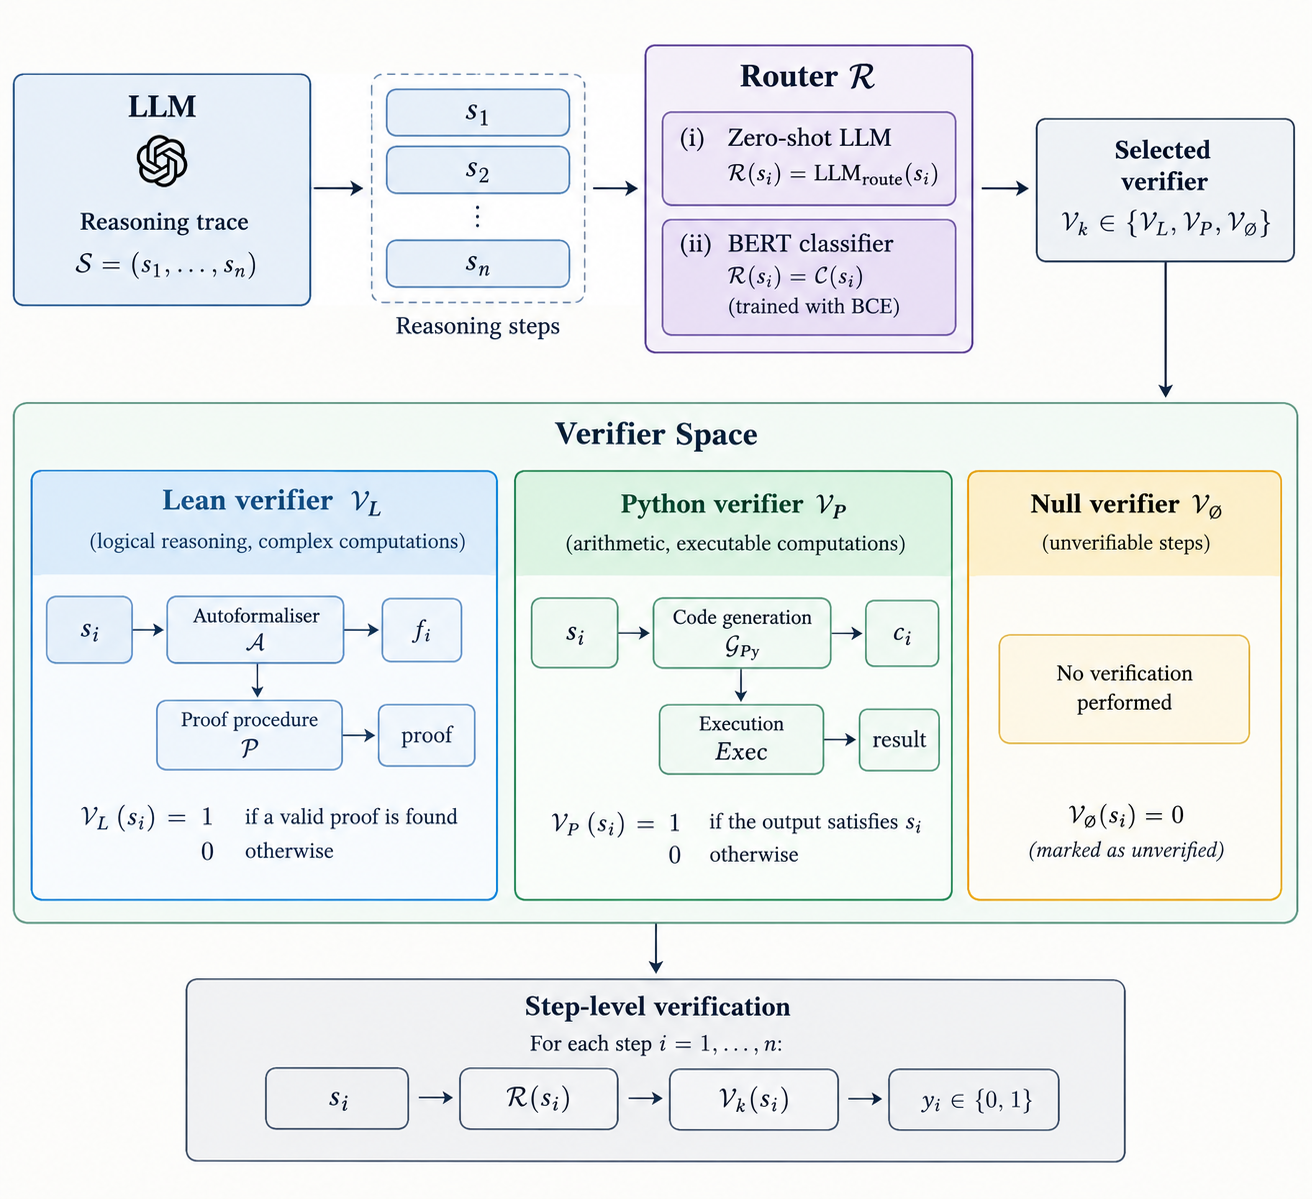
\includegraphics[width=0.85\linewidth]{sections/figures/veriform-method.png}
    \caption{Our VeriForm methodology.}
    \label{fig:placeholder}
\end{figure}

